\section{L10-Conduzione}
Per \textbf{conduzione termica} si intende la trasmissione di calore per contatto molecolare diretto. Il principio alla base della conduzione è diverso a seconda della struttura fisica del corpo: se la conduzione termica avviene nei gas è dovuta alla diffusione atomica e molecolare, se invece avviene nei liquidi e nei solidi è a causa di onde elastiche; nei materiali metallici il fenomeno è principalmente dovuto alla diffusione degli elettroni liberi dato che è trascurabile il contributo dell’oscillazione elastica del reticolo cristallino.
\subsection{Strumeti matematici}
\subsubsection{Operatore nabla}
\[
    \vec{\nabla} = \frac{\delta}{\delta x} \vec{i} + \frac{\delta}{\delta y} \vec{j} + \frac{\delta}{\delta z} \vec{k}
\]
\[
    \vec{\nabla} T = grad(T) = \frac{\delta T}{\delta x} \vec{i} + \frac{\delta T}{\delta y} \vec{j} + \frac{\delta T}{\delta z} \vec{k}
\]
\[
    \vec{\nabla} \cdot  \vec{v} = div(\vec{v}) = \frac{\delta \vec{v}_x}{\delta x} \vec{i} + \frac{\delta \vec{v}_y}{\delta y} \vec{j} + \frac{\delta \vec{v}_z}{\delta z} \vec{k}
\]
\[
    \vec{\nabla} \cdot  \vec{\nabla} T = \nabla^2 T = \;\text{laplaciano di}\;T = \frac{\delta^2 T}{\delta x^2} \vec{i} + \frac{\delta^2 T}{\delta y^2} \vec{j} + \frac{\delta^2 T}{\delta z^2} \vec{k}
\]
\subsubsection{Teorema della divergenza (o di Gauss)}
\[
    \oint_S \vec{v} \cdot \vec{n} dS = \int_{V} div(\vec{v}) dV
\]
\subsection{Equazione generale della conduzione}
Il postulato di Fourier è uno strumento incompleto ai fini della soluzione di un
problema di conduzione. Da esso però si può dedurre un'equazione
fenomenologica denominata equazione di Fourier o equazione generale della
conduzione, la cui soluzione consente di determinare la distribuzione di
temperatura in un mezzo. Questa equazione esprime il bilancio di energia di un
sistema sede di trasmissione del calore per conduzione:
\begin{center}
    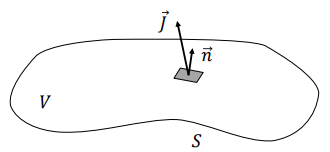
\includegraphics[height=4cm]{../L10/img2.PNG}
\end{center}
Bilancio di energia:
\[
    \frac{\delta U}{\delta t} = \dot{Q}^\leftarrow + \dot{\Sigma}
\]
dove $\frac{\delta U}{\delta t}$ è la variazione di energia nel tempo che può essere espressa in maniera più generale come $\frac{\delta}{\delta t} \int_{V} \rho u d V$ (fino ad ora nel corso abbiamo considerato situazioni in cui tutto era omogeneamente distribuito, qui però stiamo considerando casi in cui nello spazio una proprietà può variare. Con questo integrale si ottiene il valore medio), $\dot{Q}^\leftarrow$ è la potenza entrante e $\dot{\Sigma}$ è la sorgente di potenza.
\[
    \frac{\delta}{\delta t} \int_{V} \rho u d V = - \oint_S \vec{j} \cdot  \vec{n} dS + \int_{V} \sigma dV
\]
Applichiamo ora il teorema della divergenza:
\[
    \frac{\delta}{\delta t} \int_{V} \rho u dV = - \int_{V} div(\vec{j}) dV + \int_{V} \sigma dV
\]
Con le ipotesi di colume $V$ e densità $\rho$ indipendenti dal tempo si ottiene:
\[
    \int_{V} \rho \frac{\delta u}{\delta t} dV + \int_{V} div(\vec{j}) dV - \int_{V} \sigma dV = 0
\]
\[
    \int_{V}\left[\rho \frac{\delta u}{\delta t} + div(\vec{j}) - \sigma)\right]dV
\]
Per cui si ha valido per qualunque volume:
\[
    \rho \frac{\delta u}{\delta t} + div(\vec{j}) - \sigma = 0
\]
La variazione di energia interna è esprimibile attraverso la relazione $du = c_v dT$ e sfruttando inoltre il postulato di Fourier $\vec{j} = - k grad (T)$ si ottiene
\[
    \rho c_v \frac{\delta T}{\delta t} = div (k \cdot grad(T)) + \sigma
\]
con l'ipotesi di materiale omogeneo ed isotropo ($k$ costante) si ottiene l'\textbf{equazione generale della conduzione o equazione di Fourier}
\[
    \rho c_v \frac{\delta T}{\delta t} = k \nabla^2T + \sigma
\]
Questa equazione viene anche scritta come 
\[
    \frac{1}{a} \frac{\delta T}{\delta t} = \nabla^2 T + \frac{\sigma}{k}
\]
con $a = \frac{k}{\rho c_v}$ la \textbf{diffusività termica} in $[m^2/s]$.
\newline
\newline
L'equazione di Fourier è una equazione differenziale alle derivate parziali e 
\begin{itemize}
    \item lineare in $T= f(x,y,z,t)$;
    \item sel secondo ordine rispetto a $x,y,z$;
    \item del primo ordine rispetto a $t$.
\end{itemize}
\subsection{Condizioni al contorno}
L’equazione di Fourier non è risolvibile in assenza di ulteriori informazioni, quali
\begin{itemize}
    \item \textbf{condizione iniziale} (se il problema è tempo invariante);
    \item \textbf{condizioni al contorno} (o ai limiti)
\end{itemize}
\ \newline
La soluzione richiede quindi che sia \textbf{noto}:
\begin{itemize}
    \item la geometria del mezzo in cui abbiene la conduzione;
    \item le proprietà delle sorgenti termiche;
    \item la distribuzione della temperatura nel mezzo all'istante iniziale;
    \item le condizioni al contorno superficiale relative all'interazione tra il mezzo e ciò che lo delimita.
\end{itemize}
\ \newline
Per quanto riguarda le condizioni al contorno, vale la seguente \textbf{terminologia}:
\begin{itemize}
    \item \textbf{Problema di Dirichlet} (condizione di promo tipo): quando è assegnata la distribuzione della funzione $T$ (temperatura) in ogni punto del contorno, eventualmente in funzione del tempo
    \[
        T = T(\vec{x},t) \;\;\;\;\;\;\;\;\;\;\vec{x} \in S
    \]
    \item \textbf{Problema di Neumann} (condizione di secondo tipo): quando è assegnata al contorno la derivata normale della funzione $T$, eventualmente in funzione del tempo
    \[
        \frac{\delta T}{\delta \vec{n}} = f(\vec{x},t) \;\;\;\;\;\;\;\;\;\; \vec{x} \in S
    \]
    Questa condizione rappresenta, in senso fisico, la conoscenza del \textbf{flusso termico areico} alla superficie del sistema.
    \item \textbf{Problema di Cauchy} (condizione di terzo tipo): quando è assegnata al contorno una combinazione lineare della funzione $T$ e della sua derivata normale, eventualmente in funzione del tempo
    \[
        \frac{\delta T}{\delta \vec{n}} + A T = f(\vec{x}, t) \;\;\;\;\;\;\;\;\;\; \vec{x} \in S; \;\; A = \text{costante}\;
    \]
    Questa condizione si verifica nella maggior parte dei casi quando vi è scambio termico per convezione alla superficie di controllo del sistema. Si ottiene, avendo indicato con $h$ il coefficiente convettivo:
    \[
        -k \frac{\delta T}{\delta \vec{n}} = h (T-T_{\infty}) \;\;\;\;\;\;\;\;\;\; \vec{x} \in S
    \]
    essendo $T_{\infty}$ la temperatura di un eventuale fluido esterno.
    \item \textbf{Condizione di quarto tipo}: questa condizione corrisponde al caso in cui si ha scambio termico attraverso l'interfaccia di due mezzi in cui è presente un trasporto conduttivo ed aventi diversa conduttività termica ($k_1$ e $k_2$)
    \[
        -k_1 \frac{\delta T_1}{\delta \vec{n}} = -k_2 \frac{\delta T_2}{\delta \vec{n}} \;\;\;\;\;\;\;\;\;\; \vec{x} \in S
    \]
    in cui $T_1$ e $T_2$ sono le funzioni che descrivono il campo di temperatura nei mezzi rispettivamente di conduttività $k_1$ e $k_2$.\newline
    \newline
    Se il contatto tra i due mezzi materiali è perfetto, può allora essere specificata una ulteriore relazione tra le temperature superficiali dei mezzi:
    \[
        T_1 = T_2 \;\;\;\;\;\;\;\;\;\; \vec{x} \in S
    \]
\end{itemize}
\subsection{Sistema di coordinate}
